%; whizzy chapter -dvi
% -initex iniptex -latex platex -format platex -bibtex jbibtex -fmt fmt
% 以上 whizzytex を使用する場合の設定。

%     Tokyo Debian Meeting resources
%     Copyright (C) 2012 Junichi Uekawa
%     Copyright (C) 2011 Nobuhiro Iwamatsu

%     This program is free software; you can redistribute it and/or modify
%     it under the terms of the GNU General Public License as published by
%     the Free Software Foundation; either version 2 of the License, or
%     (at your option) any later version.

%     This program is distributed in the hope that it will be useful,
%     but WITHOUT ANY WARRANTY; without even the implied warranty of
%     MERCHANTABILITY or FITNESS FOR A PARTICULAR PURPOSE.  See the
%     GNU General Public License for more details.

%     You should have received a copy of the GNU General Public License
%     along with this program; if not, write to the Free Software
%     Foundation, Inc., 51 Franklin St, Fifth Floor, Boston, MA  02110-1301 USA

%  preview (shell-command (concat "evince " (replace-regexp-in-string "tex$" "pdf"(buffer-file-name)) "&"))
% 画像ファイルを処理するためにはebbを利用してboundingboxを作成。
%(shell-command "cd image201201; ebb *.png")

%%ここからヘッダ開始。

\documentclass[mingoth,a4paper]{jsarticle}
\usepackage{monthlyreport}

% 日付を定義する、毎月変わります。
\newcommand{\debmtgyear}{2013}
\newcommand{\debmtgmonth}{3}
\newcommand{\debmtgdate}{16}
% started from zero:
% (let ((year 2013) (month 3)) (+ (* (- year 2005) 12) month -1))
\newcommand{\debmtgnumber}{98}

\begin{document}

\begin{titlepage}
\thispagestyle{empty}
% タイトルページ:編集必要な部分は最初のマクロに飛ばすこと

\vspace*{-2cm}
第\debmtgnumber{}回 東京エリア Debian 勉強会資料\\
\hspace*{-2cm}

\includegraphics{image2012-natsu/dotdeb.pdf}\\
\hfill{}\debmtgyear{}年\debmtgmonth{}月\debmtgdate{}日

% ここはアップデートすること
% 全角文字にしないとフォントのサイズが合わないので注意
\rotatebox{10}{\fontsize{32}{32} {\gt 特集1:ldapvi \& python-ldap で stress-free life}}

\rotatebox{10}{\fontsize{32}{32} {\gt 特集2:gdb python 拡張}}

\vspace*{-2cm}
\hfill{}
\includegraphics[height=6cm]{image200502/openlogo-nd.eps}
\end{titlepage}

\dancersection{Introduction}{上川 純一}

\begin{multicols}{2}
 

 今月のDebian勉強会へようこそ。これからDebianの世界にあしを踏み入れると
 いう方も、すでにどっぷりとつかっているという方も、月に一回Debianについ
 て語りませんか?

 Debian勉強会の目的は下記です。

 \begin{itemize}
 \item \underline{Debian Developer} (開発者)の育成。
 \item 日本語での「\underline{開発に関する情報}」を整理してまとめ、アップデートする。
 \item \underline{場}の提供。
 \begin{itemize}
  \item 普段ばらばらな場所にいる人々が face-to-face で出会える場を提供
	する。
  \item Debian のためになることを語る場を提供する。
  \item Debianについて語る場を提供する。
 \end{itemize}
 \end{itemize}		

 Debianの勉強会ということで究極的には参加者全員がDebian Packageをがりがり
 と作るスーパーハッカーになった姿を妄想しています。情報の共有・活用を通し
 て Debianの今後の能動的な展開への土台として、「場」としての空間を提供す
 るのが目的です。

2013年の計画は下記です:
\begin{enumerate}
  \item 2013年の計画立案
 \item OSC 東京 nojima 
 \item UEFI・セキュアブートをDebianでどうやるか
 \item セキュアOS再入門
 \item Debianで自動化の夢は見れるか -- データセンターで OS のインストールからアプリのデプ
       ロイ、サービス公開まで
 \item amazon AWS での Debian 入門
 \item スイスでキャンプ
 \item Debian でスクリプト言語のパッケージ: perl, ruby, python
 \item Debian で apache 2.4: サーバ構築、Apache module プログラミング
 \item Raspberry Pi 、 SheevaBox、Freedombox は今
 \item 自由なFPGA
 \item 一年間の反省
\end{enumerate}


\end{multicols}

\newpage

\begin{minipage}[b]{0.2\hsize}
 \definecolor{titleback}{gray}{0.9}
 \colorbox{titleback}{\rotatebox{90}{\fontsize{80}{80} {\gt デビアン勉強会} }}
\end{minipage}
\begin{minipage}[b]{0.8\hsize}
\hrule
\vspace{2mm}
\hrule
\begin{multicols}{2}
\tableofcontents
\end{multicols}
\vspace{2mm}
\hrule
\end{minipage}

\dancersection{事前課題}{上川 純一}

今回の事前課題は以下です:
\begin{enumerate}
 \item Debianでここがバグってるかも?という事について列挙ください。
 \item 使ったことのある/使ってみたいデバッガについて語って下さい。
 \item LDAPのシステムを管理していますか?している場合は、slapd.confとslapd-configどちらを使っていますか?その理由は?
\end{enumerate}
この課題に対して提出いただいた内容は以下です。
\begin{multicols}{2}
{\small
 \begin{prework}{ dictoss(杉本 典充) }

\preworksection{Debianでここがバグってるかも?という事について列挙ください。}
squeezeのvirt-manager。KVM上で動作ている仮想マシンのコンソールを操作しているとき、キーボード操作でアンダースコアが入力できない。
\preworksection{使ったことのある/使ってみたいデバッガについて語って下さい。}
gdbとpdb(python)は使ったことがあります。コマンド単独で実行するより、EmacsのGUDモード内で動作させたほうがソースコードを見つつデバッグできるので効率がいいです。(eclipseを使ったときのような感じ)。sshしつつデバッグするときはGUIがないので必要に迫られて覚えた記憶があります。
\preworksection{LDAPのシステムを管理していますか?している場合は、slapd.confと
slapd-configどちらを使っていますか?その理由は?}
LDAPシステムの管理はしたことはありません。
\end{prework}

\begin{prework}{ キタハラ }

\preworksection{Debianでここがバグってるかも?という事について列挙ください。}
 今、ぱっと思いつかない。
\preworksection{使ったことのある/使ってみたいデバッガについて語って下さい。}
 最近、prinf とか syslog 程度で済むプログラムしか作っていないなぁ。
\preworksection{LDAPのシステムを管理していますか?している場合は、slapd.confと
slapd-configどちらを使っていますか?その理由は?}
していない。(実は大昔に、Netscape の Directory Server を・・・)
\end{prework}

\begin{prework}{ まえだこうへい }

\preworksection{Debianでここがバグってるかも?という事について列挙ください。}
Debian installer では LVMを使っているとパーティション情報を削除できず、shellモードから消してましたが、今ってどうなんでしょう。

\preworksection{使ったことのある/使ってみたいデバッガについて語って下さい。}
ちょっとgdb, pdbなど使ったことありますが、ちゃんと使ったがないのでそろそろ学習せんとあかんかなぁと思ってます。
\preworksection{LDAPのシステムを管理していますか?している場合は、slapd.confと
slapd-configどちらを使っていますか?その理由は?}
今回の発表内容なので割愛
\end{prework}

\begin{prework}{ たかはしもとのぶ }

\preworksection{Debianでここがバグってるかも?という事について列挙ください。}

 うーん、あまり思いつかないです。パッケージの設定が適切でないと思うことはありますが。

\preworksection{使ったことのある/使ってみたいデバッガについて語って下さい。}
  gdb もしくは Emacs + gdb を使ったことがあります。

\preworksection{LDAPのシステムを管理していますか?している場合は、slapd.confと
slapd-configどちらを使っていますか?その理由は?}
  管理しています。ファイルベースの方が扱いやすいので、どうしてもという場合以外は slapd.conf にしています。
\end{prework}

\begin{prework}{ yamamoto }

\preworksection{Debianでここがバグってるかも?という事について列挙ください。}

\begin{description}
\item [aptitude] (armehf と ppc64 では再現しているが、他のは大丈夫みたい?)
\#659341 なのだろうが、パッチを書けるほどは理解していない。

\item [ghc] (ppc64 だけかも知れないが、確認不可。多分 7.6.1-2 の頃からだと思う)
なんか特定のパッケージの特定位置で、ビルド中に固まる。
固まった時は buildd ユーザで、ssh と gcc のゾンビプロセスがいつも残っている。

\item [libccid] 日本では結構有名な NTTCom のカードリーダに関する typo。
1.4.6 でサポートされなくなり、1.4.8 で復活したが、その時 enbug した。
最近 wheezy に上げて気づいたが、BTS しないとと思いながらも、多忙によりまだ投げられてない。
\end{description}

\preworksection{使ったことのある/使ってみたいデバッガについて語って下さい。}
バグの状況説明で gdb で bt したことがあるぐらい。

\preworksection{LDAPのシステムを管理していますか?している場合は、slapd.confと
slapd-configどちらを使っていますか?その理由は?}
LDAP って、それおいしいの?
\end{prework}

\begin{prework}{ 野島 貴英 }

\preworksection{Debianでここがバグってるかも?という事について列挙ください。}
sid/experimental使ってるとそりゃもう遭遇します(←そのためのものですから無問題ですが)。\\
今も見る例:aptitudeがLANG=ja\_JP.utf8でこける事がある(再現条件不明)、gstreamer-pluginsで字幕が使えない(upstreamの問題?)、gnome-shellがたまにハング(upstreamの問題?)、gnome-keyringがまれにハング(upstreamの問題?)などなど。ただそれでも、結局Debianの問題じゃなくて、upstreamの問題のようなものばかり...\\
※Bug報告しろよという話もある。
\preworksection{使ったことのある/使ってみたいデバッガについて語って下さい。}
printf(笑)/gdb/perldb/pydb/adb/apd/xdebugなどなど。
\preworksection{LDAPのシステムを管理していますか?している場合は、slapd.confと
slapd-configどちらを使っていますか?その理由は?}
 秘密。slapd.conf直接編集かな。\\
理由:そんなに変更しないので、他の手段を使ってないだけだったりという消極的理由。
\end{prework}

\begin{prework}{ koedoyoshida }

\preworksection{Debianでここがバグってるかも?という事について列挙ください。}
debugイメージが標準で提供されていないこと。

\preworksection{使ったことのある/使ってみたいデバッガについて語って下さい。}
\begin{description}
\item [→使ったことがある] crash,lkst,gdb
\item [→使ってみたい] VisualStudio並みにグラフィカルなデバッグ環境
\end{description}
\preworksection{LDAPのシステムを管理していますか?している場合は、slapd.confと
slapd-configどちらを使っていますか?その理由は?}
過去の遺産のslapd.confのシステムが...
\end{prework}

\begin{prework}{ 鈴木崇文 }

\preworksection{Debianでここがバグってるかも?という事について列挙ください。}
あまりバグってると感じたことはないです。
\preworksection{使ったことのある/使ってみたいデバッガについて語って下さい。}
 gdbを使用したことがあります。emacs+gdbで使いやすい環境を作れたら使ってみたいです。統合開発環境としてのemacs+gdb連携ベストプラクティス的なものに興味があります。vim+gdbも試したことがありますが、結局gdbを直接使うようになってしまいました。
\preworksection{LDAPのシステムを管理していますか?している場合は、slapd.confと
slapd-configどちらを使っていますか?その理由は?}
LDAP使ったことないですね。
\end{prework}

}
\end{multicols}

\dancersection{Debian Trivia Quiz}{上川純一}

ところで、みなさん Debian 関連の話題においついていますか?Debian関連の話
題はメーリングリストをよんでいると追跡できます。ただよんでいるだけではは
りあいがないので、理解度のテストをします。特に一人だけでは意味がわからな
いところもあるかも知れません。みんなで一緒に読んでみましょう。

今回の出題範囲は\url{debian-devel-announce@lists.debian.org} や \url{debian-devel@lists.debian.org}に投稿された
内容とDebian Project Newsからです。

\begin{multicols}{2}
 %; whizzy-master ../debianmeetingresume201211.tex
% $B0J>e$N@_Dj$r$7$F$$$k$?$a!"$3$N%U%!%$%k$G(B M-x whizzytex $B$9$k$H!"(Bwhizzytex$B$,MxMQ$G$-$^$9!#(B
%

\santaku
{DebConf13 $B$N3+:ECO$H3+:EF|$O!)(B}
{$BF|K\!"El5~ET(B 6$B7n(B20$BF|(B}
{$B%K%+%i%0%"(B $B%^%J%0%"(B 7$B7n(B8-14$BF|(B}
{$B%9%$%9!"%t%)!<%^%k%-%e(B 8$B7n(B11-18$BF|(B}
{3}
{$B%K%+%i%0%"$O(BDebConf12$B$N3+:ECO$G$9!#(B
DebConf13$B$O%9%$%9$N%-%c%s%WCO$G3+:E$G$9!#(B
6/20$B$O3'$5$sM=Dj$r6u$1$F$*$-$^$7$g$&!#(B}

\santaku
{$B@$3&$N(BWeb$B%5!<%P$G:G$b?M5$$N$"$k(BLinux $B%G%#%9%H%j%S%e!<%7%g%s(B(W3Techs$BD4$Y(B)$B$O!)(B}
{CentOS}
{Debian}
{Ubuntu}
{B}
{\url{http://w3techs.com/technologies/history_details/os-linux}$B$K7k2L$N%0%i%U$,$"$j$^$9!#(B
$B8=:_(B Linux $B$r;HMQ$7$F$$$k(B web $B%5!<%P$N(B 32.9\% $B$,(B Debian $B$rMxMQ$7$F$*$j!"$=$N3d9g$O8=:_$bA}2C$rB3$1$F$$$k$=$&$G$9!#(B}

\santaku
{Debian $B%+!<%M%k%A!<%`$N%a%s%P!<$G$"$j!"(Bkernel.org $B$N(B 3.2.y $B0BDjHG7ONs$N%a%s%F%J$G$b$"$k(B Ben Hutchings $B$5$s$,<!4|(B Debian $B0BDjHG$H0l=o$K=P2Y$5$l$k(B Linux $B%+!<%M%k$K(B (3.2 $B7ONs$N(B mainline $B$K$OL5$$(B) $BDI2C5!G=$,Ek:\$5$l$kM=Dj$G$"$k$H=R$Y$F$$$^$9!#(B
$BB?$/$NDI2CE@$NCf$K4^$^$l$J$$$b$N$O2?!)(B}
{PREEMPT\_RT}
{Hyper-V guest drivers$B$N6/2=(B}
{ARM64/AArch64$B%"!<%-%F%/%A%c%5%]!<%H(B}
{C}
{Hyper-V guest drivers$B$O(Bmainline kernel$B$G(B3.2$B$K$b4^$^$l$F$$$^$9$,!"$h$j2~A1$5$l$?(B3.4$B$+$i$N=$@5$,F3F~$5$l$^$9!#(B
PREEMPT\_RT$B$O%O!<%I%j%"%k%?%$%`$r<B8=$9$k$?$a$N(BPatch$B!"(B
linux-image-rt-amd64 , linux-image-rt-686-pae $B$N(Bmetapackage$B$G;HMQ$G$-$^$9!#(B
$B?7$7$$(BARM 64$B%S%C%H%"!<%-%F%/%A%c%5%]!<%H$O(Bmainline kernel 3.7$B$+$i(B}

\santaku
{Wookey$B$5$s$,%"%J%&%s%9$7$?(Balpha$BHG$N(BDebian port arm64 image$B$O!)(B}
{Debian/Ubuntu port image}
{Debian/KFreeBSD port image}
{Debian/GnuHurd port image}
{A}
{self-bootstrapp(non x86)$BBP1~$H$N$3$H$G$9!#(B\url{http://wiki.debian.org/Arm64Port}$B$G%9%F!<%?%9$,3NG'$G$-$^$9!#(B}

\santaku
{700,000$BHVL\$N%P%0$,Js9p$5$l$?F|$rEv$F$k(B700000thBugContest$B$N7k2L$,=P$^$7$?!#$=$NM=A[F|$HJs9pF|$O!)(B}
{2012/12/12$B$rM=A[$7$?(BDavidPrevot}
{$BM=A[F|(B:2013/02/04$B!"Js9pF|(B:2013/02/14}
{$BM=A[F|(B:2013/02/07$B!"Js9pF|(B:2013/02/14}
{$BM=A[F|(B:2013/02/14$B!"Js9pF|(B:2013/02/07}
{C}
{$B:G$b6a$$(B2013/02/14$B$rM=A[$7$?(BChristian Perrier$B$5$s$,Ev$F$^$7$?!#7k2L$O(B\url{http://wiki.debian.org/700000thBugContest}$B$G8x3+$5$l$F$$$^$9!#(B
$B$^$?!"(B800,000/1,000,000$BHVL\$N%P%0$,Js9p$5$l$kF|$rEv$F$k%3%s%F%9%H(B\url{http://wiki.debian.org/800000thBugContest}$B$b3+:E$5$l$F$$$^$9!#(B}

\santaku
{master.debian.org$B$,?7$7$$5!3#$K0\9T$5$l$^$7$?!#$3$l$O2?$N%5!<%P$G$7$g$&$+(B $B!)(B}
{@debian.org$B$N%a!<%k%5!<%P(B}
{$B%Q%C%1!<%8$N%^%9%?!<%5!<%P(B}
{$B%Q%C%1!<%8$N%9%]%s%5!<(B(mentor)$B$rC5$9%5!<%P(B}
{A}
{$B8E$$%5!<%P$O%G%#%9%/>c32Ey$,$"$C$?$N$G!"<wL?$HH=CG$5$l!"%G!<%?$,B;<:$9$kA0$K?7$7$$%5!<%P$K0\9T$5$l$^$7$?!#(Bftp-master.debian.org$B$O(BDebian$B$N(B official package $B%j%]%8%H%j$G$9!#%Q%C%1!<%8$N%9%]%s%5!<(B(mentor)$B$rC5$9$N$O(Bmentors.debian.net$B!#(B }

\santaku
{pbuilder$B$K(Bclang support$B$,DI2C$5$l$^$7$?!#C/$,=q$$$?%Q%C%A$G$7$g$&$+!)(B}
{Sylvestre Ledru}
{Junichi Uekawa}
{Hideki Yamane}
{C}
{Debian$B$N(BClang$B%5%]!<%H$OCe!9$H?J$s$G$$$^$9!#(B}

\santaku
{DPN - 2013$BG/(B3$B7n(B4$BF|9f$K<h$j>e$2$i$l$?F|K\$N%$%Y%s%H$O(B}
{Open Source Conference 2013 Tokyo/Spring}
{Open Source Conference 2013 Hamamatu}
{Open Source Conference 2013 Tokushima}
{A}
{\url{http://henrich-on-debian.blogspot.jp/2013/02/open-source-conference-2013-tokyospring.html} $B>\:Y$O8e$[$I!#(B}


\end{multicols}

\dancersection{最近のDebian関連のミーティング報告}{上川純一}
\subsection{東京エリアDebian勉強会96回目報告}

2013年最初の東京エリアDebian勉強会はスクエアエニックスさんのオフィス
を間借りして開催しました。
参加者は
yy\_y\_ja\_jpさん、キタハラさん、dictossさん、koedoyoshidaさん、daiさん、
yamamotoさん、まえださん、上川さん、野島さん(+他会場お手伝い2名)
でした。

野島さん主催のDWN Quizは今回は数が少ないが難問でいい感じした。

事前課題の紹介は2015年の予想と2013年にやりたいことの提案でした。
いろいろと妄想しているのがわかりました。

全員でグループワークとして、2015年の予想、2013年の計画を行いまし
た。過去に予想した未来の確認と、あらためて今後3年間の妄想をぶつけあいま
した。

{% \tiny
\footnotesize
\begin{tabular}[t]{|p{8em}|p{14em}|p{10em}|p{8em}|p{10em}|}
%\begin{tabular}[t]{|p{8.5em}|p{12em}|p{8em}|p{6em}|p{8em}|}
\hline
2011 &2012 & 2013 & 2014 & 2015 \\
\hline
 %2011

 デスクトップパソコン終了の潮流。

 cpuコア単体では高速化しないように。

 webos終了のお知らせ。

 adobe flash復活のお知らせ(キタ), silverlight終了のお知らせ(台湾を除く)(続いてる?)

 squeezeリリース(おめでとう)

 ipv4割り当ての終了のお知らせ(キタ)

 地上波デジタル移行延長。

 btrfsまだ頑張る(fedora乙)

 java終了(sun java終了)

 open officeがoracle officeに(ナイ)

 &
 %2012

 ノートパソコンよりタブレットのほうが売れている。
 ノートパソコンではmacbookairが常識に。

 ノートパソコンでintelじゃないもの(mips/arm)が主流にはまだならず。タブレッ
 トのほうが主流。

 デスクトップ:ゲーム以外の用途では終了している。

 サーバ:個人レベルではVPS常識。企業ユースでもcloud か、vpsかを自前と比較
     検討する時代。データセンターを置く国を選べる時代。

 携帯電話:
 ガラパゴスの終焉。日本での携帯電話販売でもスマートフォンが50%を超えるように。
     ガラケー向けのネットバンクの提供が終了など、ガラケーからサービスが
     撤退し始める。
 LTE登場、普及しはじめたが、主流になっていない。
 softbankの二年契約はまだ続いている。sim freeへの道は耕されたがあたり前にならなかった。

 btrfsはまだ生き残っているがまだ使われてない?

     openstack で ceph 使う人もいる?

 mysqlからmariadbが派生。

 & 
 % 2013

コンシューマーはノートパソコンを買わなくなった。
ノートパソコンのかわりにスマートフォンを使っている。

スマートフォンが7インチくらいまで拡大、タブレットとは何だったのか。

自宅用のデスクトップパソコンのかわりに10インチくらいのタブレットを使うよ
	 うに。

サーバ:クラウドで処理するのが主流。python / ruby でコード書いていると
	 CPUが何かわからない。裏で動いているCPUは一般人は知らない。

ARMホストの仮想化技術が発達。

Oracle がメンテナンスする気がないのが明確になり、java リスクが顕著になる。

固定ゲーム機の終焉。

ゲームはARM。

 & 
 % 2014

Intel がまたARMに参入、もしくは省電力CPUを主力に切り替える。

気づいたら自作パソコン業界が終焉している。
セキュアブートが普及している。

AMD が ARM コアのCPUを出す。

Java が Oracle管理からはずれる。

スマートフォンの電池がガラケーなみに持つようになる。

電池消費が重要なアプリ選択の要素となる。
スポイトで充電できる、燃料電池が流行る。

ARメガネのプロトタイプが出てくる。

 & 
 % 2015

自作スマホの時代。
OpenHardwareがモバイルに移行する。
技適のパーツ認定基準というのができるようにがんばる。

自宅で回路が印刷できる機器が普及してCPUとかが印刷できるようになるといい
		 な。

タブレットが丸められるようになって巻物になっている。

AMD が x86 撤退。

ハードディスクを見たことがない人がいる。

データセンターを自前でもっているのは発電所を持っているところだけになる。

クラウドの法制度、免責事項、個人情報保護関連の問題が提起され、解決にむけ
		 てすすむ。
一種データセンタークラウド業者の要求規格が制定される。
ユーザ数何人以上は二種免許が必要とか。

データセンターヘイブンとよばれる国が存在する。

\\

\hline
\end{tabular}
}

そしてそのあと上川司会で2013年の各月のテーマ候補について語り合いまし
た。

最後に野島さんがDebhelperの話をして終了。
GDBの話は時間オーバーしてしまったので次回にもちこすことになりました。

\subsection{Open Source Conference 2013 Hamamatsu}

\begin{itemize}
\item 開催場所は浜松市市民協働センターさんでした。
\item 展示のみの出展で吉田、赤部さんで行いました。
\item 来場者数:約200名
\item ブース来場者数:約30名前後
\end{itemize}

\subsection{OSC Tokyo/Spring}

\begin{itemize}
\item 開催場所は明星大学さんでした。
\item セミナーは土曜日に「Debian Update」のタイトルで野島さんが行いました。
\item 展示は土曜のみ出展で吉田、やまねさん、杉本さんなどで行いました。
\item 土曜来場者数:約1000名
\item ブース来場者数:約50名前後
\end{itemize}
セミナー資料は下記で公開されています。
\url{http://www.ospn.jp/osc2013-spring/modules/article/article.php?articleid=5}
\url{http://tokyodebian.alioth.debian.org/2013-02.html}
やまねさんのリポートが下記にあります。
\url{http://henrich-on-debian.blogspot.jp/2013/02/open-source-conference-2013-tokyospring.html}


%-------------------------------------------------------------------------------
\dancersection{ldapvi \& python-ldap で stress-free life}{まえだこうへい}
%-------------------------------------------------------------------------------
\subsection{ストレス溜まってませんか?}

今回の記事はOpenLDAPの管理を行っている人がターゲットです。LDAPサーバを管理している人は多くはないと思いますが、この記事がLDAPの運用で苦労している人の一助になれば良いと思います。LDAPなにそれ?な人もLDAPアカウントやアドレス帳などで知らぬ間に恩恵を受けているということは大いにあるので、明日は我が身と思ってお読み下さい。
また、自分で作ったツールのアカウント管理をLDAPで行いたい、という場合にも参考になると思います。

なお、LDAPの基本的なお話や、DebianシステムでのOpenLDAPの入門については、第61回 関西Debian勉強会(2012年7月)に佐々木さんが発表&資料を掲載されているのでそちらを参照下さい。\footnote{あんどきゅめんてっどDebian2012年冬号8.「Debianで作るLDAPサーバ」 \url{http://tokyodebian.alioth.debian.org/pdf/debianmeetingresume2012-fuyu.pdf}}

\index{LDIF(5)}
\index{RFC2849}
\subsection{stress = LDIF}

LDAPの運用で何が面倒かというと、LDIF(LDAP Data Interchange Format)の作成やパースです。LDAPのデータを作成・更新・削除するには通常、LDIFを作成し、ldapadd/ldapmodify/ldapdeleteコマンドで実行します。一つのオブジェクトはdn(distiguised name, 識別名)から始まり、それにattributeが続きます。複数オブジェクトを記述するには空行で分割します。下記は RFC2849 の "Example 1: An simple LDAP file with two entries" からの引用です。\footnote{\url{http://www.ietf.org/rfc/rfc2849.txt}}

\begin{commandline}
version: 1
dn: cn=Barbara Jensen, ou=Product Development, dc=airius, dc=com
objectclass: top
objectclass: person
objectclass: organizationalPerson
cn: Barbara Jensen
cn: Barbara J Jensen
cn: Babs Jensen
sn: Jensen
uid: bjensen
telephonenumber: +1 408 555 1212

dn: cn=Bjorn Jensen, ou=Accounting, dc=airius, dc=com
objectclass: top
objectclass: person
objectclass: organizationalPerson
cn: Bjorn Jensen
sn: Jensen
telephonenumber: +1 408 555 1212
\end{commandline}

データフォーマット自体はさほど難しくありませんが、このデータを一から自分でスクラッチで作成するのはとても面倒だと思いませんか?例えば上記のようなユーザアカウントの場合、人間にとってはTSVなどの形式を表計算ソフトで読んだり編集したりすることでしょう。そこからLDIFに変換したり、あるいはその逆はどうしますか?簡単に思いつくのは次の二つでしょう。

\begin{enumerate}
  \item 手でちまちま変換する
  \item なんらかのプログラムで一括変換する
\end{enumerate}

前者は転記ミスなどの可能性から論外ですが、管理対象のアカウントが少数ならいっそ割り切ってLDIFを手で作成するのもありでしょう。
しかしユーザ数が大量になるとプログラムで変換しないと時間の無駄です。

\index{slapd-config(5)}
\index{OpenLDAP}
\subsubsection{そして slapd-config}
OpenLDAP 2.3からは動的に設定を変更できるslapd-config(5)が採用されました。これ自体もLDAPデータベースとなっています。current releaseの2.4系では 一部の場合のぞき、従来のslapd.conf(5)は推奨されていません。将来のリリースではslapd.conf(5)は取り除かれることになっています。\footnote{\url{http://www.openldap.org/doc/admin24/slapdconf2.html}}。廃止されるものを使いつづけても仕方ありませんね。しかし、ユーザデータの管理ですらLDIFで悩んでいるのに、さらにslapd自体の設定までもLDIFを作らないといけないと思うと、もう気が狂いそうです。

\index{ldapvi(1)}
\subsection{ldapvi で LDIF 地獄からの脱却}
そこで、ldapviです\footnote{\url{http://www.lichteblau.com/ldapvi/}}。このツールは、vipw(8)コマンドや、visudo(8)と同じように、viのインタフェースでLDAPのデータを変更できます。これで少数のデータを管理するときはもちろん、slapd-configの設定管理の悩みも解決します。

使うには、ldapviパッケージをインストールします。

\begin{commandline}
$ sudo apt-get install ldapvi
\end{commandline}

使い方は、ldap-utilsパッケージのコマンドのオプションとほぼ同じです。slapd-configでの操作は下記のコマンドを実行します。

\begin{commandline}
$ sudo ldapvi -Y EXTERNAL -h ldapi:/// -b cn=config
\end{commandline}

これでslapd-config管理下のすべてのオブジェクトツリーがldapviのフォーマットとして表示されます。ldapviのフォーマットはほぼLDIFに似ています。

\begin{commandline}
(snip)

0 cn=config
objectClass: olcGlobal
cn: config
olcArgsFile: /var/run/slapd/slapd.args
olcLogLevel: 512
olcPidFile: /var/run/slapd/slapd.pid
olcToolThreads: 1

1 cn=module{0},cn=config
objectClass: olcModuleList
cn: module{0}
olcModulePath: /usr/lib/ldap
olcModuleLoad: {0}back_hdb

2 cn=schema,cn=config
objectClass: olcSchemaConfig
cn: schema
(snip)
\end{commandline}

LDIFとの違いは、"dn: cn=config"となっている部分が"0 cn=config"と表示されていることです。この数字は表示されているオブジェクトを0を基数とする序数となっています。例えば、新しいオブジェクトを追加する場合は、数字の代わりに"add"を使います。auditlog, ppolicyモジュールを新しくロードする場合は下記のように挿入します。

\begin{commandline}
(snip)

1 cn=module{0},cn=config
objectClass: olcModuleList
cn: module{0}
olcModulePath: /usr/lib/ldap
olcModuleLoad: {0}back_hdb

add cn=modile,cn=config
objectClass: olcModuleList
cn: module
olcModulePath: /usr/lib/ldap
olcModuleLoad: auditlog.la

add cn=modile,cn=config
objectClass: olcModuleList
cn: module
olcModulePath: /usr/lib/ldap
olcModuleLoad: ppollicy.la

2 cn=schema,cn=config
objectClass: olcSchemaConfig
cn: schema
(snip)
\end{commandline}

追記したら、viと同様に保存&終了してみます(:wq コマンドを実行)。すると次のメッセージが出力されます。

\begin{commandline}
SASL/EXTERNAL authentication started
SASL username: gidNumber=0+uidNumber=0,cn=peercred,cn=external,cn=auth
SASL SSF: 0
     12 entries read                                                              
add: 2, rename: 0, modify: 0, delete: 0
Action? [yYqQvVebB*rsf+?] 
\end{commandline}

ここで、"y"を入力すると、実際にslapd-configに反映されます。前述の通り、slapd.confとは違い、slapdの再起動は不要です。"q"を入力するとキャンセルして終了します。

上記での挿入時に、 cn=module{0}の"{0}"を残したまま保存してみてください。

\begin{commandline}
add cn=modile{0},cn=config
objectClass: olcModuleList
cn: module{0}
olcModulePath: /usr/lib/ldap
olcModuleLoad: ppollicy.la
\end{commandline}

すると次のようにエラーに修正を要求されます。
\begin{commandline}
ldap_add: Naming violation (64)
add: 1, rename: 0, modify: 0, delete: 0
Action? [yYqQvVebB*rsf+?] 
\end{commandline}

これはすでに"cn=module{0}, cn=config"が存在するためです。新規追加時にdnでは親や先祖のノードに序数が指定されていれば必要ですが、自身のノードには自動的に付与されるので指定してはいけません。今回は"e"を押し編集モードに戻り、dn および attribute の cn の序数を取り除きましょう。

編集が終わったら、"y"を押して保存する前に、"v"を押します。すると、LDIF形式で表示されます。これは後々役立ちます。

\begin{commandline}
version: 1

dn: cn=module,cn=config
changetype: add
objectClass: olcModuleList
cn: module
olcModulePath: /usr/lib/ldap
olcModuleLoad: auditlog.la

dn: cn=module,cn=config
changetype: add
objectClass: olcModuleList
cn: module
olcModulePath: /usr/lib/ldap
olcModuleLoad: ppolicy.la
\end{commandline}

既にあるオブジェクトのattributeを変更する場合は、値を変更するだけです。オブジェクトを削除する場合は、対象のオブジェクトのすべての行を、特定のattributeだけを削除する場合はその行を削除するだけです。自分でLDIFを作るのと違い、非常に簡単であることがわかるでしょう。
フォーマットが間違っている場合は前述のようにエラーになる上、変更時にslapdの再起動が不要なので、実はslapd.confでの管理よりもとても便利です。

ユーザデータを変更する場合も基本的に同じです。 ldapvi コマンドで指定するオプションが異なるだけです。

\begin{commandline}
$ ldapvi -h ldap://localhost -D cn=admin,dc=example,dc=org -b dc=example,dc=org
\end{commandline}

ldapviの詳細は、ユーザマニュアルが充実しているのでそちらを参照ください。\footnote{ldapvi User Manual \url{http://www.lichteblau.com/ldapvi/manual/}}

\index{debconf}
\subsection{debconf-utils と slapd-config で導入の自動化を進める}

OpenLDAPを使う場合、slapdパッケージをインストールしますが、debconfによる対話形式の設定が必要になります。はじめてインストールする場合などには便利なのですが、ある程度なれてきて、slapd の設定自体もあらかじめ決めてあると、これはかえって面倒なものになります。予め設定するパラメータは決めてあるのですから自動化したいですよね。そういう場合debconf-utilsパッケージと、 そしてslapd-configを上手に使うことで自動化できるます。

\subsubsection{事前準備}

まず、テスト環境などを用意します。このテスト環境の目的は次の二つです。
\begin{enumerate}
  \item debconfの設定を抽出する
  \item slapd-config用のLDIFを用意する
\end{enumerate}

前者はslapdパッケージをインストールの際に今後設定したいパラメータを入力しておく必要があります。設定された状態でdebconf-utilsパッケージのdebconf-get-selectionsコマンドでslapdに関するdebconfのパラメータを抽出するためです。後者はslapdパッケージをインストールした直後の状態にしておき、この状態でldapviで予め設定したいattributeの値を変更し、前述のLDIF形式の出力します。

\subsubsection{debconf-get-selectionsでパラメータを抽出する}

slapdをインストール状態で次のコマンドを実行します。

\begin{commandline}
$ LANG=C sudo debconf-get-selections | grep slapd
slapd   slapd/password2 password
slapd   slapd/internal/generated_adminpw        password
slapd   slapd/internal/adminpw  password
slapd   slapd/password1 password
slapd   slapd/password_mismatch note
slapd   slapd/invalid_config    boolean true
slapd   shared/organization     string  example.org
slapd   slapd/upgrade_slapcat_failure   error
slapd   slapd/backend   select  HDB
slapd   slapd/dump_database     select  when needed
slapd   slapd/allow_ldap_v2     boolean false
slapd   slapd/no_configuration  boolean false
slapd   slapd/move_old_database boolean true
slapd   slapd/dump_database_destdir     string  /var/backups/slapd-VERSION
# Do you want the database to be removed when slapd is purged?
slapd   slapd/purge_database    boolean false
slapd   slapd/domain    string  example.org
\end{commandline}

このうち、"\texttt{slapd/upgrade\_slapcat\_failure}"と"\texttt{\#}"から始まるコメント行は不要です。削除してslapd-debconf.txtなどの任意のファイル名で保存します。
これをslapdパッケージのインストール時に反映させるには、パッケージインストール前にdebconf-set-selectionsコマンドを使います。

\begin{commandline}
$ sudo bash -c "cat slapd-debconf.txt | debconf-set-selections"
$ sudo DEBCONF_FRONTEND=noninteractive apt-get -y --force-yes install slapd
\end{commandline}

slapdの設定用LDIFは、前述のテスト環境でldapviを使って生成します。次の3つの設定を行います。
\begin{itemize}
\item rootDNのパスワード
\item loglevel
  \begin{itemize}
    \item 128
  \end{itemize}
\item access control
  \begin{itemize}
    \item パスワード以外のデータの参照はanonymousで可能
    \item データの更新はrootDNのみ行える
    \item パスワードのみ自身で変更可能
  \end{itemize}
\end{itemize}

\index{slappasswd}
まず、 ハッシュ化されたrootDNのパスワードをslappasswdで生成します。
\begin{commandline}
$ sudo slappasswd 
New password: 
Re-enter new password: 
{SSHA}MEj4D59lrtA+6+0J4vIz2RTByA7KT6Zq
\end{commandline}

次に、ldapviで上記の設定を行います。

\begin{commandline}
$ sudo ldapvi -h ldapi:/// -Y EXTERNAL -b cn=config
\end{commandline}

変更箇所は下記の "<- (*)" の部分です。

\begin{commandline}
0 cn=config
(snip)
olcLogLevel: 128 <- (*)
(snip)

10 olcDatabase={1}hdb,cn=config
(snip)
olcAccess: {0}to attrs=userPassword,shadowLastChange by self write by anonymous auth
 by dn="cn=admin,dc=example,dc=org" write by * none <- (*)
olcAccess: {1}to dn.base="" by * read <- (*)
olcAccess: {2}to * by dn="cn=admin,dc=example,dc=org" write by * read <- (*)
olcAccess: {3}to dn.subtree="dc=example,dc=org" by self read by * read <- (*)
olcAccess: {4}to * by * none <- (*)
(snip)
olcRootPW: {SSHA}MEj4D59lrtA+6+0J4vIz2RTByA7KT6Zq <- (*)
(snip)
\end{commandline}

変更後、LDIFを生成すると下記のように表示されます。

\begin{commandline}
version: 1

dn: cn=config
changetype: modify
replace: olcLogLevel
olcLogLevel: 128
-

dn: olcDatabase={1}hdb,cn=config
changetype: modify
replace: olcAccess
olcAccess: {0}to attrs=userPassword,shadowLastChange by self write by anonymous auth
 by dn="cn=admin,dc=example,dc=org" write by * none
olcAccess: {1}to dn.base="" by * read
olcAccess: {2}to attrs=sshPublicKey by self write
olcAccess: {3}to * by dn="cn=admin,dc=example,dc=org" write by * read
olcAccess: {4}to dn.subtree="dc=example,dc=org" by self read by * read
olcAccess: {5}to * by * none
-
replace: olcRootPW
olcRootPW: {SSHA}MEj4D59lrtA+6+0J4vIz2RTByA7KT6Zq
\end{commandline}

残念ながらldapviにはこれを任意のファイルとして保存する機能ありません。コンソールをコピーして、適当なファイル名で保存します(今回はsetup.ldif)。保存したLDIFを用い、ldapmodifyコマンドを使えばslapdサーバに反映させることができます。

\begin{commandline}
$ sudo ldapmodify -Y EXTERNAL -H ldapi:/// -f setup.ldif
\end{commandline}

パッケージのインストールから設定まで自動化するなら次のコマンドで行えます。

\begin{commandline}
sudo apt-get install debconf ldap-utils
sudo bash -c 'cat slapd-debconf.txt | debconf-set-selections'
sudo DEBCONF_FRONTEND=noninteractive apt-get -y --force-yes install slapd
ldapmodify -Y EXTERNAL -H ldapi:// -f setup.ldif
\end{commandline}

例えば、LDAP関連のツールのテストを、クリーン環境にCIなどを使って行う場合は上記のコマンドで、リポジトリにpushする度にテスト用のslapdを自動インストールしてテストを実行させることもできます。

\index{python-ldap}
\subsection{python-ldapでstress-freeに}

さらにプログラムでLDAPを扱いましょう。今回はpythonのLDAP bindingである、Python-LDAPというモジュールを使います\footnote{\url{http://www.python-ldap.org/}}。Debianではpython-ldapパッケージです。

\begin{commandline}
$ sudo apt-get install python-ldap
\end{commandline}

python-ldapで扱う基本的なデータ構造は下記のように、LDAPオブジェクトがリストになっており、
LDAPオブジェクト自体はタプルになっています。タプルの第一要素がentryDNで、第二要素が辞書になっているLDAPオブジェクトのattributesです。各attributeの値もリストになっているので、例えばobjectClassのように複数の値を持つ場合にも対応できます。そしてentryDNとattributesの各値はすべて文字列です。

\begin{commandline}
[
    ('DN', {'attribute': ['value'], 'attribute': ['value', 'value', ...], ...}),
    ('DN', {'attribute': ['value'], 'attribute': ['value', 'value', ...], ...}),
    ...
]
\end{commandline}

\subsubsection{検索(ログイン)の例}
検索の場合、指定したusernameがuidとして存在するか、存在するならsimple bindで認証できるかの処理を行っています。
\begin{commandline}
import ldap

UID = 'user0'
PASSWORD = 'passWord'

# LDAP サーバに接続
conn = ldap.initialize('ldap://localhost')
# anonymous で uid が "username" のユーザを検索
res = conn.search_s('ou=People,dc=example,dc=org', ldap.SCOPE_SUBTREE,
                    '(uid=%s)' % UID, ['uid'])
if res:
    # "username" が見つかった場合
    dn, attr_d = res[0]
    # simple bind で認証
    try:
        conn.simple_bind_s(dn, PASSWORD)
        login_result = True
    except ldap.INVALID_CREDENTIALS:
        # 認証失敗
        login_result = False
else:
    # "username" が存在しない
    login_result = False
\end{commandline}

\subsubsection{データ追加}

データの追加や更新の場合、ldap.modlistモジュールを使う必要があります。追加の場合には、ldap.modlist.addModList()を使いますが、前述の辞書型のattributesを引数にすると、下記のフォーマットのリストに変換されます。
\begin{commandline}
[('attribute', ['value']),
 ('attribute', ['value', 'value', ...]), ...]
\end{commandline}

これを\texttt{ldap.add\_s(dn, attrs\_l)}の引数とすれば新規オブジェクトの追加ができます。サンプルは次の通りです。

\begin{commandline}
import ldap.modlist

rootdn = 'cn=admin,dc=example,dc=org'
rootpw = 'password'

dn = 'uid=mkouhei,ou=People,dc=example,dc=org'
attrs_d = {'objectClass': ['inetOrgPerson', 'posixAccount', 'shadowAccount'],
           'uidNumber': ['1000'],
           'gidNumber': ['1000'],
           'homeDirectory': ['/home/mkouhei'],
           'loginShell': ['/bin/bash'],
           'uid': ['mkouhei'],
           'cn': ['Kouhei'],
           'sn': ['Maeda']}

# attributes を辞書からリストに変換
attrs_l = ldap.modlist.addModlist(attrs_d)
# rootdn で bind
conn.simple_bind_s(rootdn, rootpw)
# dn を指定して新規オブジェクトを追加
conn.add_s(dn, attrs_l)
\end{commandline}

\subsubsection{データの削除}

データを削除する場合は、dn を指定するだけです。

\begin{commandline}
conn.delete_s(dn)
\end{commandline}

\subsubsection{python-ldap の筆者の使用例}
サーバ/ネットワークまわりの自動化ツールや、ユーザ向けのWebベースのツールの開発をpythonで行っています。認証にはLDAPを使うことが多いため、これらのツール用にpython-ldapを使ったモジュールを作っています。
また、複数の異なるLDAPアカウントのツリーをマージするのにも使っています。ユーザアカウントのデータを変換してマージする必要があるため、LDIFを自分でパースして変換するのではなく、pythonのリストや辞書で処理できるのはとても楽です。変換元のLDAPサーバには標準スキーマではなく独自拡張のスキーマを使っているものあり、名前すら違うattributeもあるのでpythonで処理できるのが大変便利です。

\subsection{まとめ}
ldapvi、python-ldapを使うとLDIFを自分で作成したり、パースする必要がなくなることを説明しました。 また、slapd-config であってもldapviを使えば、slapd.confでの場合と同様に簡単に管理できることも説明しました。注意点としては、slapd.conf での設定パラメータの名前がslapd-configでは多少異なることですが、cn=configのツリーのrootを指定すると、 ロードされているスキーマも見ることができるのでそこから検索、類推することができます。ストレスフルな LDAP の管理を少しでも stress-free にできるようになると良いですね。

\begin{thebibliography}{0}
  \bibitem{rfc2849} RFC2849 "Example 1: An simple LDAP file with two entries" \url{http://www.ietf.org/rfc/rfc2849.txt}
  \bibitem{openldap} OpenLDAP Software 2.4 Administrator's Guide \url{http://www.openldap.org/doc/admin24/index.html}
  \bibitem{ldapvi} ldapvi User Manual, \url{http://www.lichteblau.com/ldapvi/manual/}
  \bibitem{python-ldap} python-ldap Documentation, \url{http://www.python-ldap.org/doc/html/index.html}
\end{thebibliography}

%-------------------------------------------------------------------------------
\dancersection{gdb python拡張その1}{野島 貴英}
%-------------------------------------------------------------------------------
%$

\index{gdb-pythonかくちょう@gdb-python拡張}
\subsection{はじめに}

 Debianパッケージのバイナリのバグ潰しを行う時、gdbなどのデバッガを使ってデバッグを
する事も多いかと思います。しかしながら、プログラムの構造が大規模/複雑になってくると、
デバッグ作業も大変になっていきます。また、プログラムについても、
抽象化が激しく行われていると、デバッガ無しには解析が非常に困難かと思います。

 gdbはv7.0からpython拡張が搭載されており
\footnote{\url{http://ftp.gnu.org/gnu/gdb/}調べ}、gdbをpythonスクリプトで操る
事ができます。こちらを利用する事により、人手では、工数かかりすぎでなかなか
進まなかったデバッグも可能になっていくと思います。

 今回は、gdbのpython拡張の一部を説明し、最後はC言語で作られた
プログラムの実行トレースを実際にpython拡張機能を用いて、取得してみる
ところまでやってみます。

\subsection{Debian sidのgdb python拡張の基本情報}

 debian sidに含まれているgdbは最初からpython拡張が有効にしてあるようです。
表\ref{tab:gdb-python-basic-info}に基本情報を載せます。

\begin{table}[ht]
\begin{center}
\small
\begin{tabular}{|l|l|l|}
\hline
項番 & 項目 & 値 \\
\hline
1 & gdbバージョン & 7.4.1 \\
2 & pythonバージョン & 2.7.3 \\
3 & pythonサーチパス & /usr/share/gdb/python,/usr/lib/python2.7以下 \\
\hline
\end{tabular}
\caption{Debian sid環境に含まれるgdbとpythonの基本情報}
\label{tab:gdb-python-basic-info}
\end{center}
\end{table}

 今回はdebian sid amd64環境でテストした結果を元に説明を行います。

\subsection{python拡張を簡易的に動かしてみる}

 gdbよりpython言語を簡易的に呼び出す場合、gdbのコマンドラインから接頭辞として
pythonをつけて起動します。また、gdbコマンドラインから
pythonのみを指定すると、Ctrl+dを押下するまで、複数のpython構文を
指定できます。(なお、Ctrl+dを押下すると、gdbのコマンドラインに復帰する
と同時に入力した複数のpython構文が一度に評価されます)

 なお、pythonで一度定義した変数などはgdbを終了するまで何度でも
参照できます。

\begin{commandline}
$ gdb 
GNU gdb (GDB) 7.4.1-debian
Copyright (C) 2012 Free Software Foundation, Inc.
...中略...
For bug reporting instructions, please see:
<http://www.gnu.org/software/gdb/bugs/>.
(gdb) python print "hello world"
hello world
(gdb) python a=[1,2,3,4]
(gdb) python print a
[1, 2, 3, 4]
(gdb) python a.append(5)
(gdb) python print a
[1, 2, 3, 4, 5]
(gdb) python
>import sys
>print sys.path
>print sys.version_info
>ここでCtrl+d
['/usr/share/gdb/python', '/usr/lib/python2.7',
  '/usr/lib/python2.7/plat-linux2', '/usr/lib/python2.7/lib-tk',
  '/usr/lib/python2.7/lib-old', '/usr/lib/python2.7/lib-dynload',
  '/usr/local/lib/python2.7/dist-packages',
  '/usr/lib/python2.7/dist-packages',
  '/usr/lib/python2.7/dist-packages/PIL',
  '/usr/lib/python2.7/dist-packages/gst-0.10',
  '/usr/lib/python2.7/dist-packages/gtk-2.0',
  '/usr/lib/pymodules/python2.7']
sys.version_info(major=2, minor=7, micro=3, releaselevel='final', serial=0)
\end{commandline}
% $ 
\subsection{gdbのpython拡張の構造}

 gdbのpython拡張は図\ref{fig:python-internal-schema}のような構造となっています。

\begin{figure}[h]
\begin{center}
 \includegraphics[width=0.8\hsize]{image201301/gdb-python/gdb-python-internal-schema.eps}
 \caption{gdbとpython拡張の構造}
 \label{fig:python-internal-schema}
\end{center}
\end{figure}

\subsection{module gdbのマニュアル}

 gdb本体にmodule gdbが実装されているため、module gdbの
pythonドキュメントについては、gdb上でpythonからhelp(gdb)を呼び出す必要
があります。

 以下に読み方を示します。なお、以降、(gdb)はgdbのプロンプトを示します。

\begin{commandline}
(gdb) python help(gdb)
Help on package gdb:

NAME
    gdb

FILE
    (built-in)

PACKAGE CONTENTS
    command (package)
    printing
    prompt
    types

...中略...
\end{commandline}

 また、gdbのpython拡張についてのさらに詳しい説明は、info gdbにて
Extending GDB→pythonの項目から参照できます。

\subsection{module gdbに定義されているオブジェクト群}

 図\ref{fig:python-class-schema-1}〜図\ref{fig:python-class-schema-2}に、
module gdbに定義されているオブジェクト群のclass図を載せます。

 gdb拡張用のpythonスクリプトを記載する場合、これらオブジェクトを併用して
gdbとのデータのやりとり、あるいは、操作を行います。

\begin{figure}[h]
\begin{center}
 \includegraphics[width=0.8\hsize]{image201301/gdb-python/gdb-python-class-schema-1.eps}
 \caption{module gdbのclass図(その1)}
 \label{fig:python-class-schema-1}
\end{center}
\end{figure}

\begin{figure}[h]
\begin{center}
 \includegraphics[width=0.8\hsize]{image201301/gdb-python/gdb-python-class-schema-2.eps}
 \caption{module gdbのclass図(その2)}
 \label{fig:python-class-schema-2}
\end{center}
\end{figure}

\newpage

\subsection{gdbのコマンドを増やしてみる}

 gdbのpython拡張は柔軟な機能を持つため、いろいろな使い方ができます。
ここでは、試しにgdbのコマンドを増やしてみます。

 gdbのコマンドをpythonから増やすには、gdb.commandクラスを継承したクラスを
用意し、gdb.command.\_\_init\_\_()にてコマンド名と共に登録する事により行います。

 info gdbのExtending GDB→Python→Python API→Commands In Pythonに
記載されている方法を試して、hello-worldコマンドを登録してみます。

\begin{commandline}
-----hello.pyの中身ここから-----
# -*- coding: utf-8 -*-
# coding:utf-8
import gdb
class HelloWorld (gdb.Command):
  """ Greet the whole world """
  def __init__ (self):
     super(HelloWorld, self).__init__ ("hello-world",gdb.COMMAND_OBSCURE)

  def invoke (self,arg, from_tty):
     print "Hello, World! arg=["+str(arg)+"]"

HelloWorld()
-----hello.pyの中身ここまで-----
\end{commandline}

 追加したコマンドについていろいろ実行してみます。

\begin{commandline}
(gdb) source hello.py
(gdb) hello-[ここでTABを押すと補完される]
(gdb) hello-world foo,bar,com
Hello, World! arg=[foo,bar,com]
(gdb) help obscure
Obscure features.

List of commands:

...中略...
hello-world --  Greet the whole world 
...中略...
\end{commandline}

 コマンド hello-worldが追加されています。また、引数はinvoke()のargに文字列として
まとめて入ります。また、コマンドカテゴリのOBSCUREに登録されている事がhelp obscure
にて判ります。

\subsection{作ったpythonスクリプトを自動で読み込ませるには}

 ところで、gdbのpython拡張を理解するにつれ、高度なデバッグ用スクリプトを用意するように
なってくると思います。すると、作ったpythonスクリプトをいつもgdbに自動で読み込ませ
ておきたくなるかと思います。方法としては、以下の3つの方法があります。

\subsubsection{\$\{HOME\}/.gdbinitを使う方法}

 以下のようなファイルを\verb!${HOME}/.gdbinit!に記載しておきます。

\begin{commandline}
----${HOME}/.gdbinitここから-----
source /home/foo/bar/my-gdb-func.py
----${HOME}/.gdbinitここまで-----
\end{commandline}

こうすると、\verb!${HOME}!にホームディレクトリがあるようなユーザがgdbを起動した時に、
自動的に/home/foo/bar/my-gdb-func.pyがロードされて評価されるようになります。

\subsubsection{セクション名:.debug\_gdb\_scriptsを使う方法}

 バイナリ形式によりますが、任意のセクション名を持つ事が可能なバイナリ形式
(例:ELF,DWARF)にて、.gdb\_gdb\_scriptsセクションを作成し、ここにスクリプト名
を打ち込んでおく事ができる場合があります。この場合、カレントディレクトリにある、
同名のスクリプトをgdbが自動的にロードしてくれます。
なお、本機能は、gdb変数のauto-load-scriptがonの時に有効です(デフォルトはon。)

 以下に例を示します。ここでは先ほどのhello.pyを自動でロードするように
asm\{\}命令で.debug\_gdb\_scriptsセクションを直接指定しています。

\begin{commandline}
------hello.cの中身ここから------
#include <stdio.h>

asm(
".pushsection \".debug_gdb_scripts\",\"MS\",@progbits,1\n"
".byte 1\n"
".asciz \"hello.py\"\n"
".popsection \n"
);

int main(int argc,char **argv)
{
        printf("hi there!");
        return 0;
}
------hello.cの中身ここまで------

実行結果:
$ gcc -o hello hello.c
$ ls 
hello hello.py hello.c
$ gdb hello
GNU gdb (GDB) 7.4.1-debian
Copyright (C) 2012 Free Software Foundation, Inc.
...中略...
<http://www.gnu.org/software/gdb/bugs/>...
Reading symbols from /home/xxxx/hello...done.
(gdb) info auto-load-scripts
Loaded  Script                                                                 
Yes     hello.py                                                         
	full name: /home/xxxx/hello.py
(gdb) hello-world 
Hello, World! arg=[]
\end{commandline}
%$

\subsubsection{``バイナリ名''-gdb.pyをスクリプト名に使う方法}

 ファイル名として、``バイナリ名''-gdb.pyをファイル名に持つpythonスクリプトを
カレントディレクトリに置いておくと、gdbがバイナリ名のファイルをロードした時、
自動でロードしてくれます。なお、本機能は、gdb変数のauto-load-scriptがonの時に
有効です(デフォルトはon)

 以下の例では、gdb helloとすると、無事先ほどのhello.pyが読み込まれ、
hello-worldコマンドが登録されている事がわかります。

\begin{commandline}
------hello.cの中身ここから------
#include <stdio.h>

int main(int argc,char **argv)
{
        printf("hi there!");
        return 0;
}
------hello.cの中身ここまで------

コンパイル:
$ gcc -o hello hello.c
$ mv hello.py hello-gdb.py (←先ほどのhello.pyの名前を"バイナリ名"-gdb.pyへ変更)
$ ls 
hello hello-gdb.py hello.c
$ gdb hello
GNU gdb (GDB) 7.4.1-debian
Copyright (C) 2012 Free Software Foundation, Inc.
...中略...
<http://www.gnu.org/software/gdb/bugs/>...
Reading symbols from /home/xxxx/hello...done.
(gdb) info auto-load-scripts
Loaded  Script                                                                 
Yes     /home/xxxx/hello-gdb.py
(gdb) hello-world 
Hello, World! arg=[]
\end{commandline}
%$

\subsection{break/finishと応用例について}

 デバッガの基本機能にbreakpointがあります。こちらの機能を
pythonから利用するには gdb.Breakpoint class及び、
gdb.FinishBreakpoint classを継承する事により行います。
これらclassを用いれば、gdbのbreak/watch/finishコマンドを独自拡張できます。

 ここでは、応用としてバイナリ内部の関数呼び出しの記録を取るようなpythonスクリプト
を書いてみます。

\begin{commandline}
-------calltracer.pyここから---------
# -*- coding: utf-8 -*-
# coding:utf-8
import gdb
class _CallTracerFinishBreakpoint(gdb.FinishBreakpoint):
	def __init__(self, name, stack):
		super(_CallTracerFinishBreakpoint, self).__init__(internal=True)
		self._stack_ptr=stack
		self._name=name
		self.silent=True
	def stop(self):
		print (" " * (len(self._stack_ptr)))+"<="+self._name
		self._stack_ptr.pop()
		return False
	def out_of_scope(self):
		print "Abnormal jump out frame"
		print (" " * (len(self._stack_ptr)))+"<="+self._name
		self._stack_ptr.pop()
		return False

class _CallTracerBreakpoint(gdb.Breakpoint):
	def __init__(self, spec, name, stack):
		super(_CallTracerBreakpoint, self).__init__(spec, 
							    gdb.BP_BREAKPOINT,
							    internal = False)
		self._stack_ptr=stack
		self._name=name
		self.silent=True
	def stop(self):
		self._stack_ptr.append(self._name)
		print (" " * (len(self._stack_ptr)))+"=>"+self._name
		try:
			_CallTracerFinishBreakpoint(self._name, self._stack_ptr)
		except:
			print "uh? cant put finish break on "+self._name
		return False

class _ReAnalyzeCallTracer(gdb.Command):
	""" reanalyze symbol for calltracer """
	def __init__(self):
		super(_ReAnalyzeCallTracer, self).__init__('reanalyzecalltracer',
							gdb.COMMAND_OBSCURE)
		self._stack=[]
	def _retrive_ptrs(self):
		info=gdb.execute("info break",False, True)
		info_lines=info.splitlines()
		ptrs={}
		for idx in range(0,len(info_lines[1:])):
			tokens=info_lines[idx+1].split()
			if len(tokens) > 5:
				if ptrs.has_key(tokens[4]) == False:
					ptrs[tokens[4]]=" ".join(tokens[5:])
		return ptrs
	def invoke(self, arg, from_tty):
		break_info=self._retrive_ptrs()
		gdb.execute("delete",False, True)
		gdb.execute("set pagination off")
		for addr,name in break_info.iteritems():
			_CallTracerBreakpoint(r'*'+addr,
					      name,self._stack)
_ReAnalyzeCallTracer()

class _PrepareCallTracer(gdb.Command):
	""" prepare call tracer for c """
	def __init__(self):
		super(_PrepareCallTracer, self).__init__('prepcalltracer',
							 gdb.COMMAND_OBSCURE)
	def invoke(self, arg, from_tty):
		gdb.execute("rbreak",False, True)
		gdb.execute("reanalyzecalltracer",False, True)
		print "prepare done!"

_PrepareCallTracer()
-------calltracer.pyここまで---------
-------デバッグ対象:chkfunc.c ここから-------
#include<stdio.h>

void foo_a(const char *str)
{
	printf("%s\n",str);

}
void caller_bar(void)
{
	foo_a("caller is bar!");
}
int main(int argc,char **argv)
{
	foo_a("caller is main!");
	caller_bar();
	return(0);
}
-------デバッグ対象:chkfunc.c ここまで-------
\end{commandline}
\begin{commandline}
実行結果:
$ gcc -O0 -g -o chkfunc chkfunc
$ ls
chkfunc.c chfunc calltracer.py
$ gdb ./chkfunc
GNU gdb (GDB) 7.4.1-debian
Copyright (C) 2012 Free Software Foundation, Inc.
...中略...
Reading symbols from /home/foo/bar/chkfunc...done.
(gdb) source calltracer.py
(gdb) prepcalltracer 
prepare done!
(gdb) run
Starting program: /home/foo/bar/chkfunc 
 =><_start>
uh? cant put finish break on <_start>
  =><__libc_start_main@plt>
   =><__libc_csu_init>
    =><_init>
     =><call_gmon_start>
     <=<call_gmon_start>
    <=<_init>
    =><frame_dummy>
     =><register_tm_clones>
     <=<frame_dummy>
    <=<register_tm_clones>
   <=<__libc_csu_init>
   =>in main at chkfunc.c:21
uh? cant put finish break on in main at chkfunc.c:21
    =>in foo_a at chkfunc.c:12
     =><puts@plt>
caller is main!
     <=<puts@plt>
    <=in foo_a at chkfunc.c:12
    =>in caller_bar at chkfunc.c:17
     =>in foo_a at chkfunc.c:12
      =><puts@plt>
caller is bar!
      <=<puts@plt>
     <=in foo_a at chkfunc.c:12
    <=in caller_bar at chkfunc.c:17
    =><__do_global_dtors_aux>
     =><deregister_tm_clones>
     <=<deregister_tm_clones>
    <=<__do_global_dtors_aux>
    =><_fini>
    <=<_fini>
[Inferior 1 (process 6413) exited normally]
Abnormal jump out frame
   <=<__libc_start_main@plt>
warning: Error removing breakpoint -5
(gdb)
\end{commandline}
%$

無事、バイナリ内部の関数呼び出しの記録が取れているかと思います。

\subsection{終わりに}

 今回gdbのpython拡張のいくつかを紹介してみました。pythonを
用いる事で、いろいろなデバッグ手法が取れるかと思います。

 次回は、Frame class/Value class等の応用について紹介したいと思います。

\begin{thebibliography}{98}
\bibitem{infogdb} Free Software Foundation, ``info gdb''
\bibitem{gdbpytutor} ``PythonGdbTutorial'',\url{http://sourceware.org/gdb/wiki/PythonGdbTutorial}
\bibitem{gdbpytest} Free Software Foundation, \verb!$(GDBSRC)/gdb/testsuite/gdb.python!以下のテスト用ファイル群
\end{thebibliography}

\dancersection{月刊Debhelper dh\_auto\_install dh\_install}{吉田 俊輔}

\subsection{今月のコマンド}
{\Large
\begin{itemize}
\item dh\_auto\_install
\item dh\_install
\end{itemize}
}

\subsection{debian パッケージ構築、全体の流れ}
2011年10月勉強会資料より
\begin{enumerate}
\item パッケージビルド環境を構築する
\item 不要なファイルを削除する
\item バイナリパッケージに格納するファイルをビルドする
\item ビルドしたファイルをバイナリパッケージにまとめる
\item .changesファイルを作成する
\item パッケージに署名する
\end{enumerate}


\subsection[containsverbatim]{4. ビルドしたファイルをバイナリパッケージにまとめる}
\begin{itemize}

\item 以下のdebhelper コマンドが実行されます。
\begin{commandline}
dh_testdir -> dh_auto_configure -> dh_auto_build -> dh_auto_test
-> dh_testroot -> dh_prep -> dh_installdirs -> dh_auto_install
-> dh_install -> dh_installdocs -> dh_installchangelogs
-> dh_installexamples -> dh_installman -> dh_installcatalogs
-> dh_installcron -> dh_installdebconf -> dh_installemacsen
-> dh_installifupdown -> dh_installinfo -> dh_pysupport
-> dh_installinit -> dh_installmenu -> dh_installmime
-> dh_installmodules -> dh_installlogcheck -> dh_installlogrotate
-> dh_installpam -> dh_installppp -> dh_installudev -> dh_installwm
-> dh_installxfonts -> dh_installgsettings -> dh_bugfiles -> dh_ucf
-> dh_lintian -> dh_gconf -> dh_icons -> dh_perl -> dh_usrlocal
-> dh_link -> dh_compress -> dh_fixperms -> dh_strip -> dh_makeshlibs
-> dh_shlibdeps -> dh_installdeb -> dh_gencontrol -> dh_md5sums
-> dh_builddeb
\end{commandline}
\end{itemize}

\subsection{dh\_auto\_install動作解説}

dh\_auto\_installはdebhelperのプログラムです。
自動的にファイルをパッケージ作成用のディレクトリにインストールします。
dh\_auto\_installはupstearm等のMakefileのinstallターゲット,setup.py,
Build.PLのを使用して、
インストール先はシングルバイナリ(only one binary package)であれば、
debian/package/以下です。
multiple binary packageの場合はdebian/tmp/以下になり、
その後dh\_installで適切なディレクトリに移動されます。
\includegraphics[height=3cm]{image201303/dh_auto_install1.eps}

\begin{itemize}
\item 条件1:Makefile(またはsetup.pyやBuild.PL)が GNU の慣例に準拠し、\$(DESTDIR) 変数をサポートしていること。
\end{itemize}
\url{http://www.gnu.org/prep/standards/html\_node/DESTDIR.html\#DESTDIR}
\\
Makefile ファイルを変更する必要があるなら、これら \$(DESTDIR) 変数をサポートするように注意しましょう。
\begin{itemize}
\item 条件2:インストール先の指定内容が Filesystem Hierarchy Standard (FHS) に準拠していること。
\end{itemize}
\url{http://www.debian.or.jp/community/devel/debian-policy-ja/policy.ja.html/ch-opersys.html}

通常プログラムのビルドに使われているmake等を使って実際のインストール先のかわりに、一時ディレクトリーの下に作成されたファイルツリーのイメージへプログラムをインストール(コピー)する。
 普通のプログラムインストールとDebian パッケージ作成というこれら二つの違いには、debhelper パッケージの dh\_auto\_configure と dh\_auto\_install のコマンドを使うことで(前述の条件を守っていれば、特に意識をせずに)対応できるはずです。
GNU autoconf を使っているプログラムは、自動的に GNU 規約に準拠するので、そのパッケージ作成は簡単にできる(はず)。
\url{http://www.debian.org/doc/manuals/maint-guide/modify.ja.html}


\subsection[containsverbatim]{override例}
マルチパッケージで、DESTDIRを使っていないのでoverrideで対応する例(wide-dhcpv6
\begin{commandline}
override_dh_auto_install:
        $(MAKE) prefix=$(CURDIR)/debian/tmp/usr install
\end{commandline}
この後、dh\_installで各パッケージに振り分け(後述)


\subsection{dh\_install動作概要}

dh\_installはパッケージ構造ディレクトリーへインストールするファイルを扱うdebhelperプログラムです。
これ以外に多くのdh\_install*コマンドが存在します。説明書(documentation),サンプル(examples),マニュアルページ(man pages)のような特定のタイプのファイルのインストールにはするにはそれら専用のプログラムの方が向いています。


\subsection{dh\_install動作概要2}
二つの使用方法があります。
\begin{itemize}
\item upstearmのMakefileがインストールを行ってくれないとき、適所へそれらをコピーさせるために使用する。
\item 複数のバイナリパッケージを構築するラージ・パッケージを構築するとき
\end{itemize}

\newpage

\subsection{dh\_install*コマンド(debhelper内)}
\begin{table}[htb]
\scalebox{1}[1]{
\begin{tabular}{|l|r|} \hline
コマンド & 行数 \\ \hline
dh\_installcatalogs - install and register SGML Catalogs & 126 \\ \hline
dh\_installchangelogs - install changelogs into package build directories & 181 \\ \hline
dh\_installcron - install cron scripts into etc/cron.* & 87 \\ \hline
dh\_installdeb - install files into the DEBIAN directory & 118 \\ \hline
dh\_installdebconf - install files used by debconf in package build directories & 136 \\ \hline
dh\_installdirs - create subdirectories in package build directories & 96 \\ \hline
dh\_installdocs - install documentation into package build directories & 311 \\ \hline
dh\_installemacsen - register an Emacs add on package & 134 \\ \hline
dh\_installexamples - install example files into package build directories & 116 \\ \hline
dh\_installifupdown - install if-up and if-down hooks & 79 \\ \hline
dh\_installinfo - install info files & 87 \\ \hline
dh\_installinit - install init scripts and/or upstart jobs into package build directories & 287 \\ \hline
dh\_installlogcheck - install logcheck rulefiles into etc/logcheck/ & 76 \\ \hline
dh\_installlogrotate - install logrotate config files & 60 \\ \hline
dh\_installman - install man pages into package build directories & 268 \\ \hline
dh\_installmanpages - old-style man page installer (deprecated) & 207 \\ \hline
dh\_installmenu - install Debian menu files into package build directories & 99 \\ \hline
dh\_installmime - install mime files into package build directories & 105 \\ \hline
dh\_installmodules - register modules with modutils & 134 \\ \hline
dh\_installpam - install pam support files & 69 \\ \hline
dh\_installppp - install ppp ip-up and ip-down files & 75 \\ \hline
dh\_installtex - register Type 1 fonts, hyphenation patterns, or formats with TeX & 664 \\ \hline
dh\_installudev - install udev rules files & 125 \\ \hline
dh\_installwm - register a window manager & 118 \\ \hline
dh\_installxfonts - register X fonts & 97 \\ \hline
\end{tabular}
}
\end{table}

\subsection{ラージ・パッケージの構築}
(dh\_auto\_installまたはoverride\_dh\_auto\_install等を使用して)debian/tmpへすべてインストール。
そこから適切なパッケージディレクトリーを構築するためにディレクトリーやファイルをdh\_installを使用してコピーすることができます。
\\
debhelper互換性レベル7から、カレント・ディレクトリ(あるいは--sourcedirオプションで指定したディレクトリ)に対象が無ければ、dh\_installはdebian/tmpをコピー元に使用します。
debian/package.installに
各パッケージへインストールするべきファイル、およびそれらがインストールされるべきディレクトリーを記載します。
フォーマットは、行単位でインストールするべきファイル(複数可)をリストし、行の末尾にそれがインストールされるべきディレクトリーを記載します。\\
要するにcpコマンドの引数です。
\\
実際にdh\_install内部ではcpコマンドが使用されています。


\subsection[containsverbatim]{debian/package.installの例}

\begin{commandline}
$ cat wide-dhcpv6-client.install
usr/sbin/dhcp6c
usr/sbin/dhcp6ctl
debian/dhcp6c.conf etc/wide-dhcpv6
debian/scripts/dhcp6c-script etc/wide-dhcpv6
debian/scripts/dhcp6c-ifupdown etc/wide-dhcpv6
\end{commandline}

明示的なコピー先なしで、一行に1つのファイル名あるいはワイルドカード・パターンを単独で記載すると、dh\_installが自動的に使用する目的地を推測する。
これは--autodestオプションの動作と同様。


\subsection[containsverbatim]{--autodest オプション}
コピー先ディレクトリを推測する。
これを指定する場合、debian/package.installファイルのコピー先ディレクトリは指定しないこと。
debian/tmpのディレクトリ配下にあるファイルをdebian/tmpを除いて
指定ディレクトリの下に対応するようにコピーする。
例 
\begin{commandline}
$ cat debian/package.install
debian/tmp/usr/bin
debian/tmp/etc/passwd
\end{commandline}
debian/tmp/usr/binをdebian/package/usr/へコピー
debian/tmp/etc/passwdをdebian/package/etc/へコピー


\subsection{--list-misqqsing オプション}
ファイル(およびシンボリックリンク)がどのディレクトリにもコピーされなかったときに標準エラー出力に警告を表示する。
\\
ラージ・パッケージに、新しく追加されたファイルを見逃さないためなどに使える。


\subsection{-Xitem, --exclude=item オプション}
指定したファイル名を含むファイルをコピー対象外とする。

\newpage

\subsection[containsverbatim]{DEBHELPERのプログラム共通のオプション1}
アーキティクチャ独立
\begin{table}[htb]
\scalebox{1}[1]{
\begin{tabular}{|l|p{30em}|} \hline
-i, --indep & Act on all architecture independent packages. \\ \hline
\end{tabular}
}
\end{table}

例
\begin{commandline}
$ dh_make -m --rulesformat old
\end{commandline}
\begin{commandline}
install-indep:
	(中略)
        dh_prep -i 
        dh_installdirs -i
	(中略)
        dh_install -i
	(後略)
\end{commandline}


\subsection[containsverbatim]{DEBHELPERのプログラム共通のオプション2}
アーキティクチャ依存
\begin{table}[htb]
\scalebox{1}[1]{
\begin{tabular}{|l|p{30em}|} \hline
-s, --same-arch & This used to be a smarter version of the -a flag, but the -a flag is now equally smart. \\ \hline
-a, --arch & Act on architecture dependent packages that should be built for the build architecture. \\ \hline
\end{tabular}
}
\end{table}
\\
例(同)
\begin{commandline}
install-arch:
	(中略)
        dh_prep -s 
        dh_installdirs -s

        # Add here commands to install the arch part 
        # of the package into debian/tmp.
        $(MAKE) DESTDIR=$(CURDIR)/debian/hello install

        dh_install -s
	(後略)
\end{commandline}

\newpage
\subsection{DEBHELPERのプログラム共有のオプションその他}
\begin{table}[htb]
\scalebox{1}[1]{
\begin{tabular}{|l|p{30em}|} \hline
オプション & 動作 \\ \hline
-v, --verbose & 詳しく動作を表示(Verbose mode: show all commands that modify the package build directory.) \\ \hline
--no-act & 実際の動作をしない(Do not really do anything. If used with -v, the result is that the command will output what it would have done.) \\ \hline
-ppackage, --package=package & Act on the package named package. This option may be specified multiple times to make debhelper operate on a given set of packages. \\ \hline
-Npackage, --no-package=package & Do not act on the specified package even if an -a, -i, or -p option lists the package as one that should be acted on.  \\ \hline
--remaining-packages & Do not act on the packages which have already been acted on by this debhelper command earlier (i.e. if the command is present in the package debhelper log).  For
           example, if you need to call the command with special options only for a couple of binary packages, pass this option to the last call of the command to process
           the rest of packages with default settings. \\ \hline
--ignore=file & Ignore the specified file. This can be used if debian/ contains a debhelper config file that a debhelper command should not act on. Note that debian/compat,
           debian/control, and debian/changelog can't be ignored, but then, there should never be a reason to ignore those files.
           For example, if upstream ships a debian/init that you don't want dh\_installinit to install, use --ignore=debian/init  \\ \hline
-Ptmpdir, --tmpdir=tmpdir & Use tmpdir for package build directory. The default is debian/package \\ \hline
--mainpackage=package & This little-used option changes the package which debhelper considers the "main package", that is, the first one listed in debian/control, and the one for which
           debian/foo files can be used instead of the usual debian/package.foo files. \\ \hline
-O=option|bundle & This is used by dh(1) when passing user-specified options to all the commands it runs. If the command supports the specified option or option bundle, it will
           take effect. If the command does not support the option (or any part of an option bundle), it will be ignored.\\ \hline
\end{tabular}
}
\end{table}


%\printindex

\cleartooddpage

\vspace*{15cm}
\hrule
\vspace{2mm}

\includegraphics[width=2cm]{image200502/openlogo-nd.eps}
\noindent \Large \bf Debian 勉強会資料\\
\noindent \normalfont \debmtgyear{}年\debmtgmonth{}月\debmtgdate{}日 \hspace{5mm}  初版第1刷発行\\
\noindent \normalfont 東京エリア Debian 勉強会 (編集・印刷・発行)\\
\hrule

\end{document}
